\documentclass[UTF8,zihao=-4]{ctexart}
\usepackage[a4paper,margin=2.5cm]{geometry}
\usepackage{amsmath, amssymb, amsthm}
\usepackage{bm}
\usepackage{hyperref}
\usepackage{graphicx}
\usepackage{caption}
\usepackage{listings}
\usepackage{xcolor}
\usepackage{float}
\usepackage{placeins}
\graphicspath{{figures/}}

% Code style
\lstdefinestyle{code}{
  basicstyle=\ttfamily\small,
  numbers=left,
  numberstyle=\tiny,
  numbersep=8pt,
  keywordstyle=\color{blue},
  commentstyle=\color{teal!70!black},
  stringstyle=\color{orange!70!black},
  showstringspaces=false,
  breaklines=true,
  frame=single,
  framerule=0.3pt,
  rulecolor=\color{black!15}
}
\lstset{style=code}

\title{注意力机制与 Transformer 详解}
\author{}
\date{\today}

\begin{document}
\maketitle

\section{注意力机制的动机与公式}
注意力机制让模型在生成输出时聚焦关键输入。设查询 $\mathbf{Q}$、键 $\mathbf{K}$、值 $\mathbf{V}$,加性注意力的得分为
\begin{equation}
  e_{ij} = \mathbf{v}^{\top} \tanh(\mathbf{W}_q \mathbf{q}_i + \mathbf{W}_k \mathbf{k}_j),
\end{equation}
而缩放点积注意力计算为
\begin{equation}
  \mathrm{Attention}(\mathbf{Q}, \mathbf{K}, \mathbf{V}) = \mathrm{softmax}\left( \frac{\mathbf{Q} \mathbf{K}^{\top}}{\sqrt{d_k}} \right) \mathbf{V}.
\end{equation}
Softmax 权重可自适应地强调重要元素。图~\ref{fig:attention_scores_cn} 示意了注意力如何重分配关注。

\subsection{对齐与上下文向量}
在序列到序列任务中,注意力通过 $\mathbf{c}_i = \sum_j \alpha_{ij} \mathbf{v}_j$ 构造上下文向量,缓解编码器瓶颈并支持变长输入。

\subsection{变体}
常见变体包含加性(Bahdanau)注意力、乘性(Luong)注意力和位置注意力。单调注意力适用于语音识别等需要保持顺序的场景;稀疏或硬注意力选择 Top-$k$ 元素以提高效率。

\section{Self-Attention 与 Multi-Head Attention}
Self-Attention 在同一序列内计算 $\mathbf{Q}$、$\mathbf{K}$、$\mathbf{V}$,可捕捉长程依赖。多头注意力将输入投影到多个子空间并并行计算:
\begin{align}
  \mathrm{head}_i &= \mathrm{Attention}(\mathbf{Q} \mathbf{W}_i^Q, \mathbf{K} \mathbf{W}_i^K, \mathbf{V} \mathbf{W}_i^V), \\
  \mathrm{MHA}(\mathbf{Q}, \mathbf{K}, \mathbf{V}) &= \mathrm{Concat}(\mathrm{head}_1, \ldots, \mathrm{head}_h) \mathbf{W}^O.
\end{align}
多头机制能学习到不同语法或位置关系。图~\ref{fig:self_attention_heads_cn} 展示了多头注意力的关注模式。

\subsection{位置编码}
因自注意力对顺序不敏感,Transformer 需引入位置编码。正弦编码使用固定频率:
\begin{align}
  \mathrm{PE}_{(pos, 2i)} &= \sin\left( \frac{pos}{10000^{2i/d_{\text{model}}}} \right), \\
  \mathrm{PE}_{(pos, 2i+1)} &= \cos\left( \frac{pos}{10000^{2i/d_{\text{model}}}} \right).
\end{align}
也可采用可学习位置嵌入或旋转位置编码(RoPE),提升外推能力。

\subsection{效率挑战}
自注意力的复杂度为 $\mathcal{O}(n^2)$。稀疏注意力、局部注意力或线性注意力(Performer、Linformer)通过近似或限制接收域来降低长序列开销。

\section{Transformer 架构}
Transformer 编码器-解码器由多层堆叠组成,每层包含多头注意力与前馈网络。编码器层执行:
\begin{align}
  \mathbf{z} &= \mathrm{LayerNorm}(\mathbf{x} + \mathrm{MHA}(\mathbf{x})), \\
  \mathbf{y} &= \mathrm{LayerNorm}(\mathbf{z} + \mathrm{FFN}(\mathbf{z})),
\end{align}
其中 FFN 为逐位置的两层 MLP,激活通常取 ReLU 或 GELU。解码器在自注意力外还包含交叉注意力,以利用编码器输出。残差连接与层归一化保证深层网络稳定。

\subsection{前馈网络变体}
FFN 一般将隐藏维度扩展(如 512→2048)再投影回原维度。GLU、SwiGLU 或深度可分离卷积能增强表达能力。Dropout、随机深度等正则化手段缓解过拟合。

\subsection{训练策略}
Transformer 依赖大规模数据与并行计算。常用技巧包括标签平滑、学习率 warmup、Adam/Adafactor、自适应梯度累积与混合精度训练。

\begin{figure}[H]
  \centering
  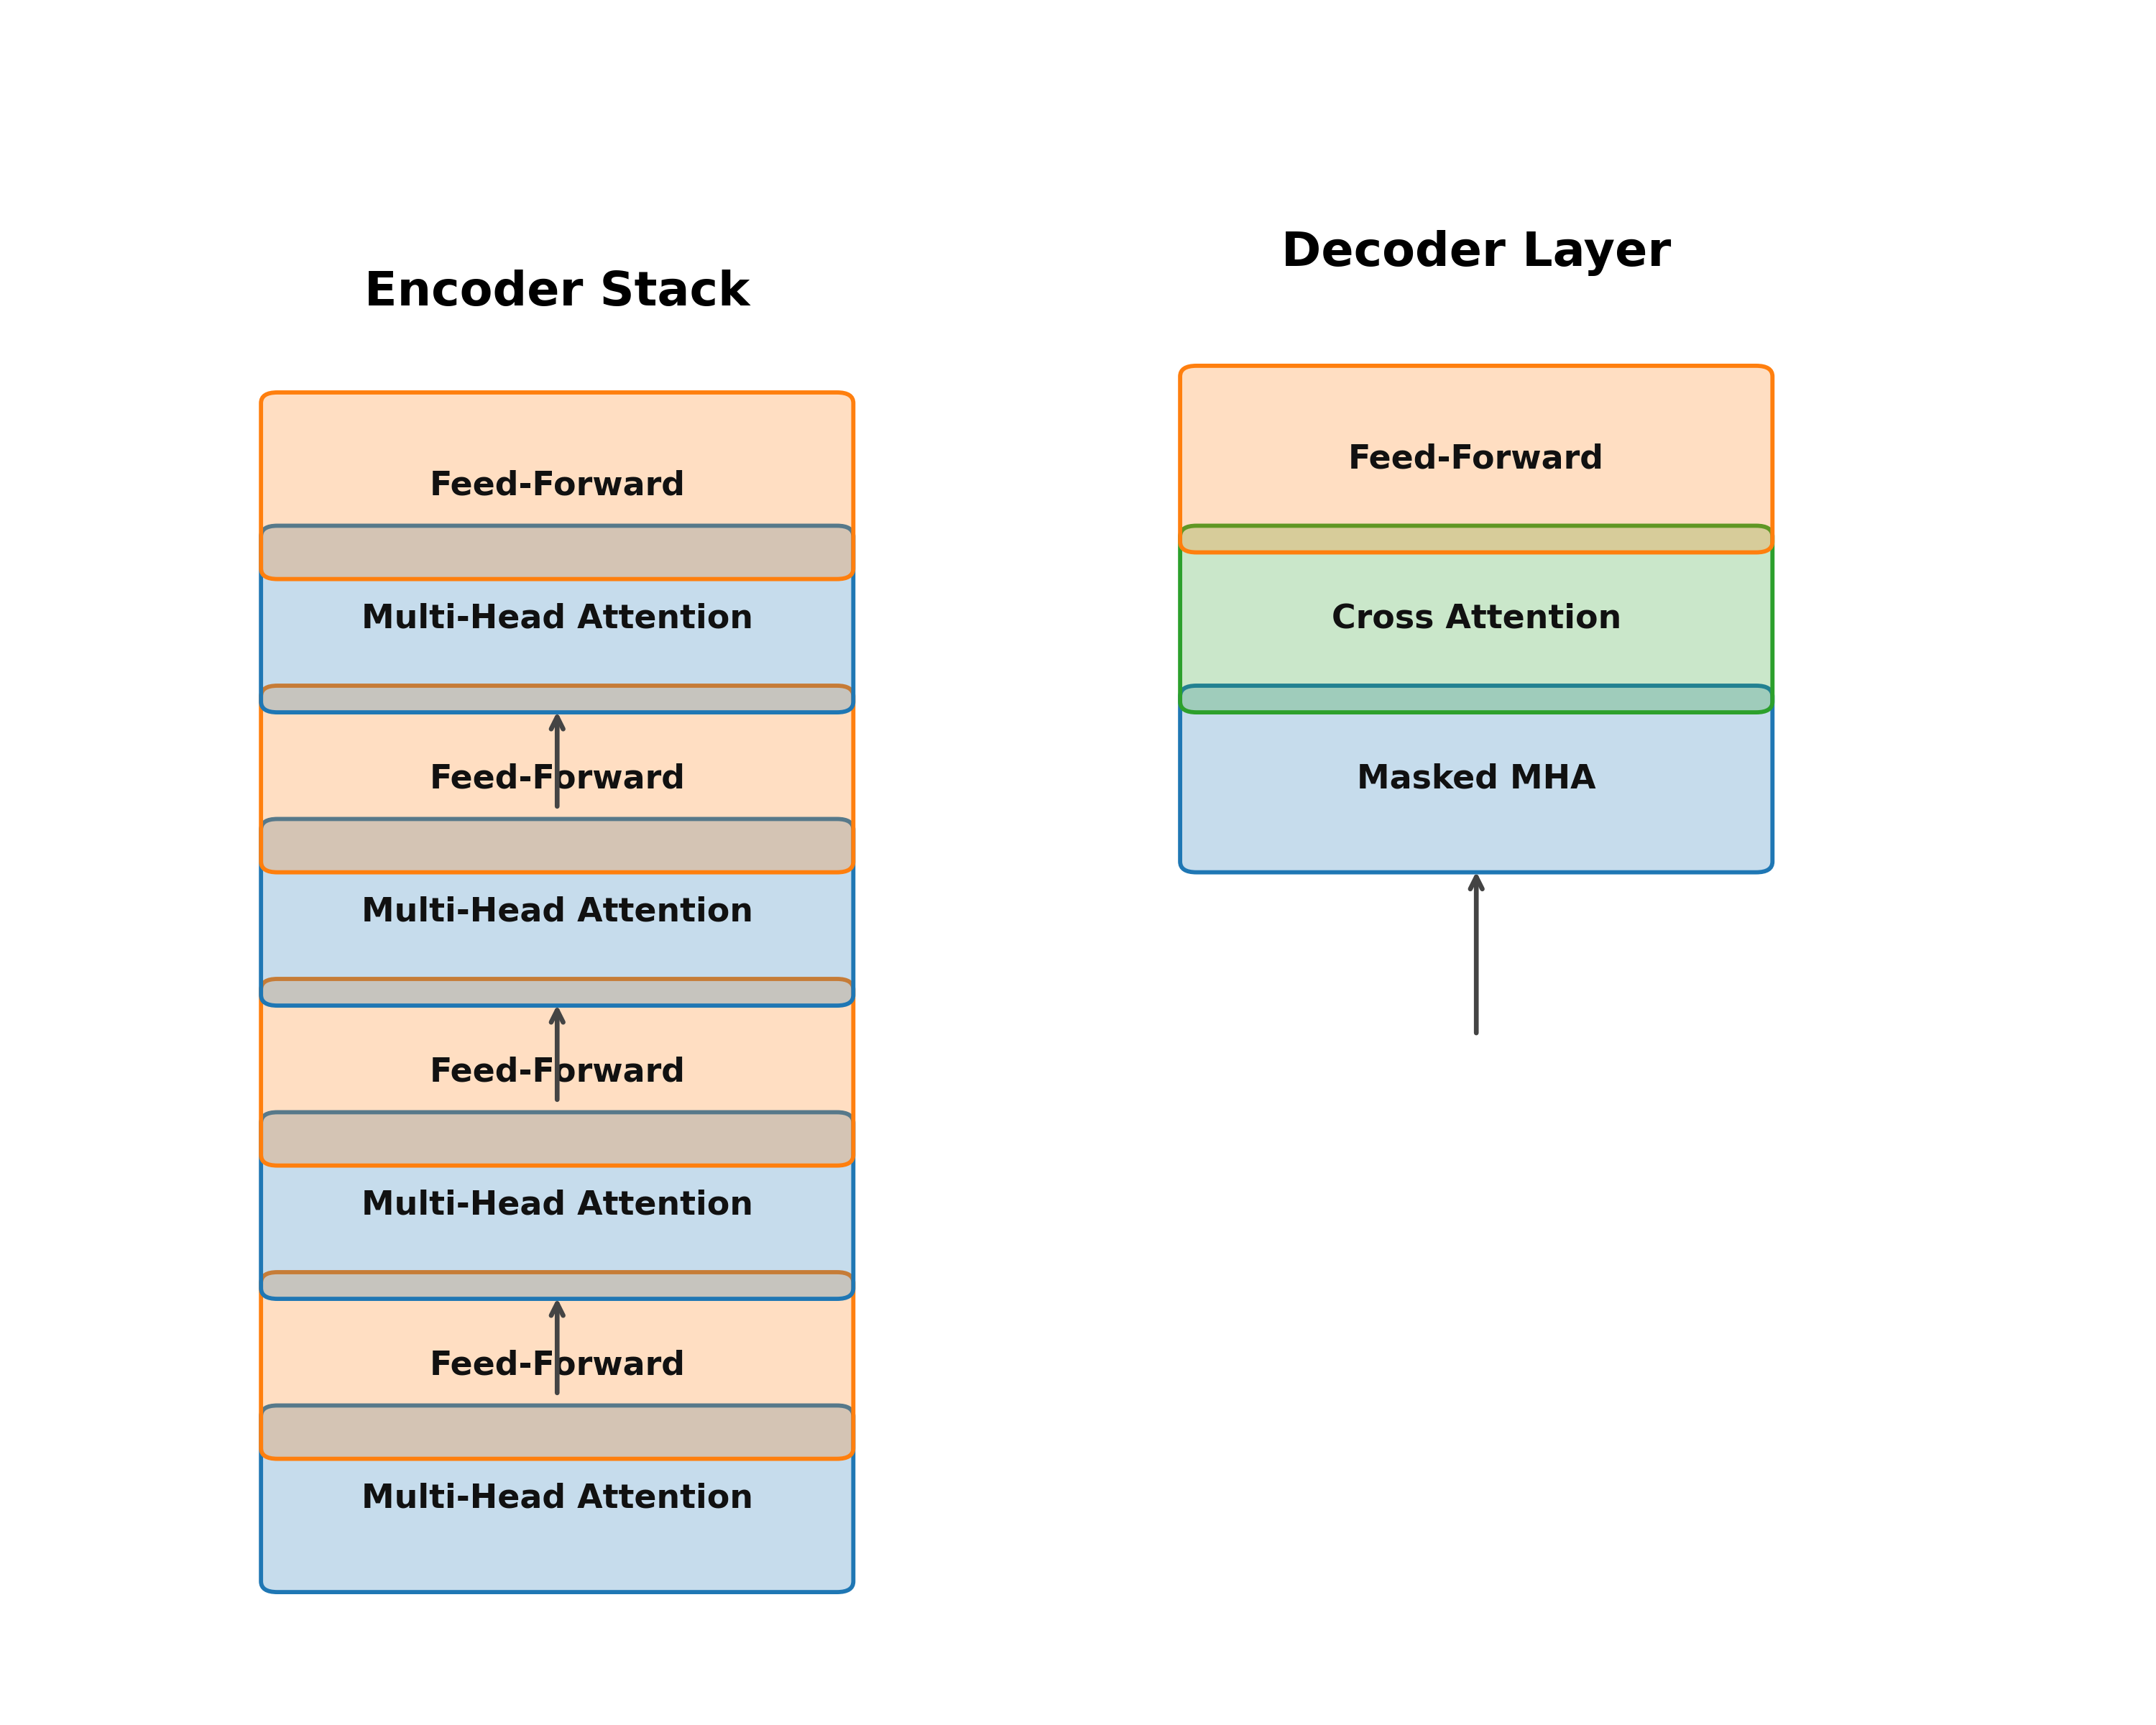
\includegraphics[width=0.85\linewidth]{transformer_layer_stack.png}
  \caption{Transformer 编码器-解码器结构:自注意力、交叉注意力与前馈网络。}
  \label{fig:transformer_stack_cn}
\end{figure}
\FloatBarrier

\section{BERT 与 GPT 系列}
预训练 Transformer 彻底改变了自然语言处理。

\subsection{BERT}
BERT 通过遮盖语言模型(MLM)与下一句预测(NSP)任务进行预训练,仅使用编码器堆叠并采用双向自注意力。微调时在 [CLS] 上添加任务特定层即可适配分类、问答等任务。

\subsection{GPT 系列}
GPT 采用解码器结构,以自回归语言模型目标训练:给定历史上下文预测下一个 token。规模化规律表明模型越大性能越好。GPT-2/3 展示了零样本与小样本提示能力,GPT-4 更进一步引入多模态输入与工具调用。

\subsection{对比与扩展}
BERT 擅长理解类任务(分类、抽取),GPT 擅长生成。T5、BART 等模型统一编码器-解码器目标。指令微调、人工反馈强化学习(RLHF)、检索增强等进一步提升效果。

\section{应用:NLP 与跨模态学习}
注意力与 Transformer 支撑了现代 AI 系统。

\subsection{自然语言处理}
Transformer 主导机器翻译、摘要、情感分析、问答等任务。预训练编码器为检索系统提供上下文向量;序列到序列 Transformer 支撑神经机器翻译与抽象摘要。

\subsection{跨模态与多模态}
Vision Transformer 将图像切分为 patch 进入自注意力。CLIP 通过对比预训练对齐文本与图像。视频 Transformer 建模时空依赖,音频 Transformer 处理语音识别与音乐生成。多模态大模型整合视觉、文本、音频实现具身推理。

\subsection{知识注入}
检索增强模型(RAG)、记忆增强 Transformer、Adapter 等结构可引入外部知识。Prompt Tuning 与 LoRA(低秩适配)提供参数高效微调方案。

\begin{figure}[H]
  \centering
  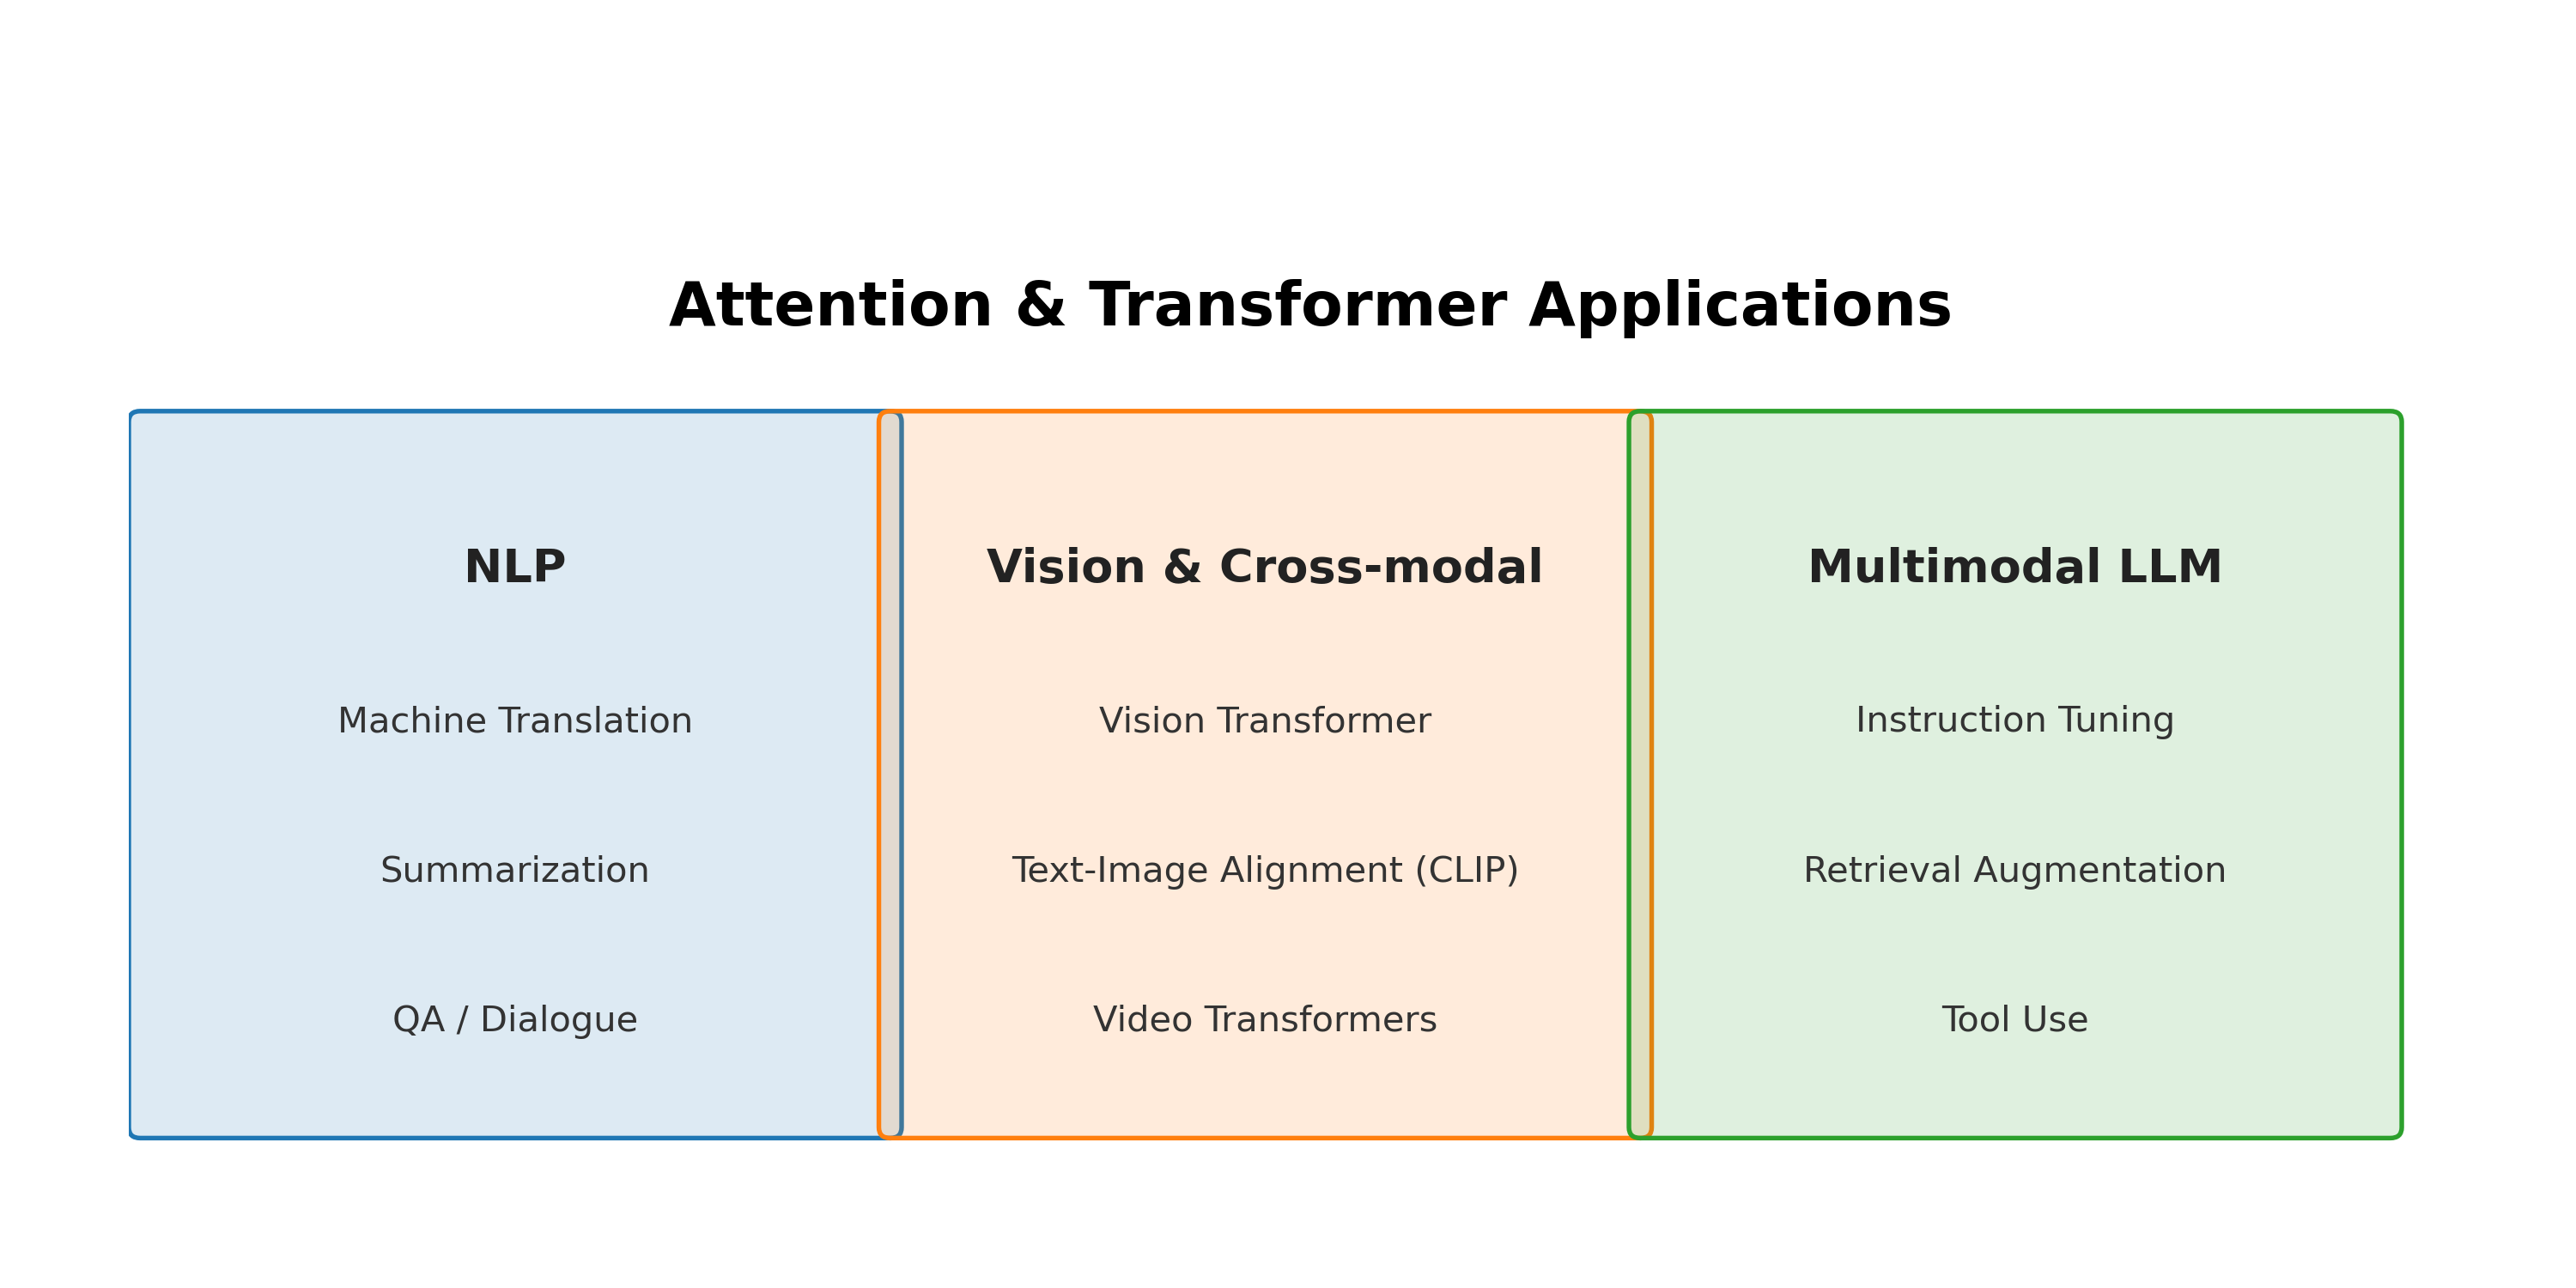
\includegraphics[width=0.85\linewidth]{attention_transformer_applications.png}
  \caption{注意力与 Transformer 在 NLP 与多模态场景中的应用。}
  \label{fig:transformer_applications_cn}
\end{figure}
\FloatBarrier

\section{实践建议}
\begin{itemize}
  \item \textbf{内存管理:} 采用梯度检查点、混合精度、序列分块处理长序列。\item \textbf{正则化:} 使用 dropout、注意力 dropout、标签平滑、权重衰减。\item \textbf{规模化:} 参考损失缩放规律,调整批量、学习率调度(余弦+warmup)与梯度裁剪。\item \textbf{评估:} 根据任务关注 BLEU、ROUGE、准确率、困惑度,并分析注意力图与校准。\item \textbf{部署:} 通过蒸馏、量化、稀疏注意力等技术压缩模型以满足延迟需求。\end{itemize}

\end{document}
